\section{Model-Based Testing}

Model-based testing is a software testing technique that uses test generation algorithms and a behavioral model of the system under test to generate test cases~\cite{1200168} and itdepends on three
key technologies~\cite{Dalal1999}: the notation used for the data model,
the test-generation algorithm, and the tools that generate supporting
infrastructure for the tests.

Unlike traditional testing techniques which tend to focus on implementation,
model-based testing stresses the use of models at all levels of the process~\cite{5381477}.
Like the data-driven and keyword-driven approaches to testing, model-based
testing relies heavily on abstraction. However, the definition of a model varies
greatly, depending on the approach~\cite{Jääskeläinen2008}. One crucial thing
that we should be aware about model-based testing is that the derived test cases
are only as good as the information in the model from which they are derived.

\begin{figure}[!ht]
\centering
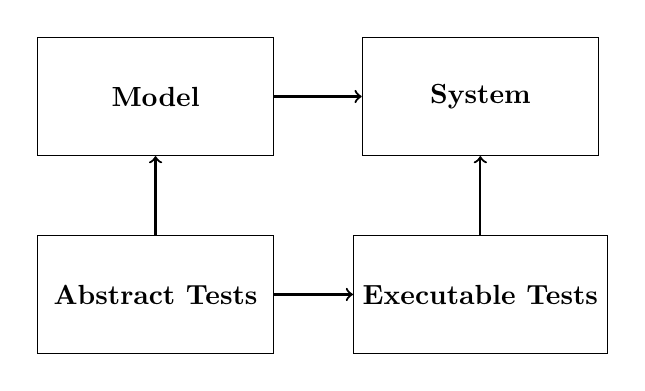
\begin{tikzpicture}
\matrix [column sep=10mm, row sep=10mm] {
  \node (model) [draw, shape=rectangle, minimum width=3cm, minimum height=1.5cm] {\textbf{Model}}; & \node (system) [draw, shape=rectangle, minimum width=3cm, minimum height=1.5cm] {\textbf{System}}; \\
  \node (abstests) [draw, shape=rectangle, minimum width=3cm, minimum height=1.5cm] {\textbf{Abstract Tests}}; & \node (exectests) [draw, shape=rectangle, minimum width=3cm, minimum height=1.5cm] {\textbf{Executable Tests}}; \\
};
\draw[->, thick] (abstests) -- (model);
\draw[->, thick] (exectests) -- (system);
\draw[->, thick] (model) -- ([yshift=-5mm]system);
\draw[->, thick] (abstests) -- ([yshift=-10mm]exectests);
\end{tikzpicture}
\caption{The model is a partial description of the system under test, the abstract tests are derived from the model, and the executable tests are the concrete implementation of the abstract tests that can be run against the system under test.} \label{fig:f3}
\end{figure}

Instead of writing hundreds of test cases the test designer writes an abstract
model of the system under test, and then the model-based testing tool generates
a set of test cases from that same model. It allow to easily generate a large
test suite from the same model or regenerate the test suite each time the system
requirements change. By following this approach, the test design time is reduced
and several test suites can be generated by just using different test criteria.
The purpose of model-based testing is to solve problems~\cite{1200168} that
other testing processes do not fully address like:
\begin{itemize}
\item Automation of the design of functional test cases to reduce the design cost;
\item Produce test suites with systematic coverage of the model;
\item Reduction of the maintenance costs of the test suite;
\item Automatic generation of the traceability matrix from requirements to test cases.
\end{itemize}
Still, it offers considerable promise in reducing the cost of test generation,
increasing the effectiveness of the tests, and shortening the testing cycle.
Test generation can be especially effective for systems that are changed
frequently, because testers can update the data model and then rapidly
regenerate a test suite, avoiding tedious and error-prone editing of a suite of
hand-crafted tests~\cite{Dalal1999}.

\subsection{Model notations}

The ideal model notation would be easy for testers to understand, describe a
large problem as easily as a small system, and still be a form understood by a
test-generation tool~\cite{Dalal1999}. 

There are several modeling notations that have been used for modeling the
functional behavior of systems~\cite{1200168}: 

\begin{itemize}
\item \textbf{State-based notations}: These notations model a system as a collection of
variables, which represent a snapshot of the internal state of the system, plus
some operations that modify those variables.
\item \textbf{Transition-based notations}: These notations focus on describing the
transitions between different states of the system. Typically, they are
graphical notations, such as finite state machines, where the nodes represent
the major states of the system and the arcs represent the actions or operations
of the system.
\item \textbf{History-based notations}:  These notations model a system by
describing the allowable traces of its behavior over time. Various notions of
time can be used, leading to many kinds of temporal logics. Although they are
used as a basis for model-based testing they are better used for visualizing the
tests that result from model-based testing than for defining the model that is
the input to model-based testing.
\item \textbf{Functional notations}: These notations describe a system as a
collection of mathematical functions. Algebraic specifications tend to be more
abstract and more difficult to write than other notations, so they are not
widely used for model-based testing.
\item \textbf{Operational Notations}: These notations describe a system as a
collection of executable processes, executing in parallel. They are particularly
suited to describing distributed systems and communications protocols.
\item \textbf{Stochastic Notations}: These notations describe a system by a
probabilistic model of the events and input values. They tend to be used to model
environments rather than systems under test. They are good for specifying
distributions of events and test inputs for the system under test but are
generally weak at predicting the expected outputs.
\item \textbf{Data-flow notations}: These notations concentrate on the flow of
data through the system under test, rather than its control flow.
\end{itemize}

There is no ideal modeling language for all purposes, which implies that several
notations may be required~\cite{Dalal1999}. However, state-based notations are
best for data-oriented systems and transition-based
notations are best for control-oriented systems~\cite{1200168} but the system
could not be so easy to classify and it can be a mix of both data and
control-oriented. Choosing the wrong notation could make the system harder to
model. A good choice should be the right balance between the notation tooling
support and what notation suits the system best. It is important to build
an accurate model, written in a formal modeling notation that has precise
semantics and unambiguous meaning in order to allow different tools to
understand and manipulate the model behaviour.

\subsection{How to model a system?}

The first and most important step in modeling a system for testing is deciding the level of abstraction of the model. It should be clear which aspects of the system under test to include in the model and which aspects to omit. We should always have in mind that a smaller model is often more useful than a large and complex model, since it allow us to test each one of them independently and think about which operations should be included before writing a model for the whole system. 

When modeling a system is also important to think about the data that it manages, the operations that it performs, and the subsystems that it communicates with. The difficulty of test generation is usually highly dependent on the number and range of the input parameters, so applying the same abstraction principle~\cite{Mosley2002} to its input and output parameters helps to control the test generation effort.

The next step is to decide which notation to use for the model. This decision is
often influenced by the model-based testing tools that are available and the
notations they support. It is important to consider which style of notation is
most suitable for the system under test.

\begin{figure}[!ht]
\centering
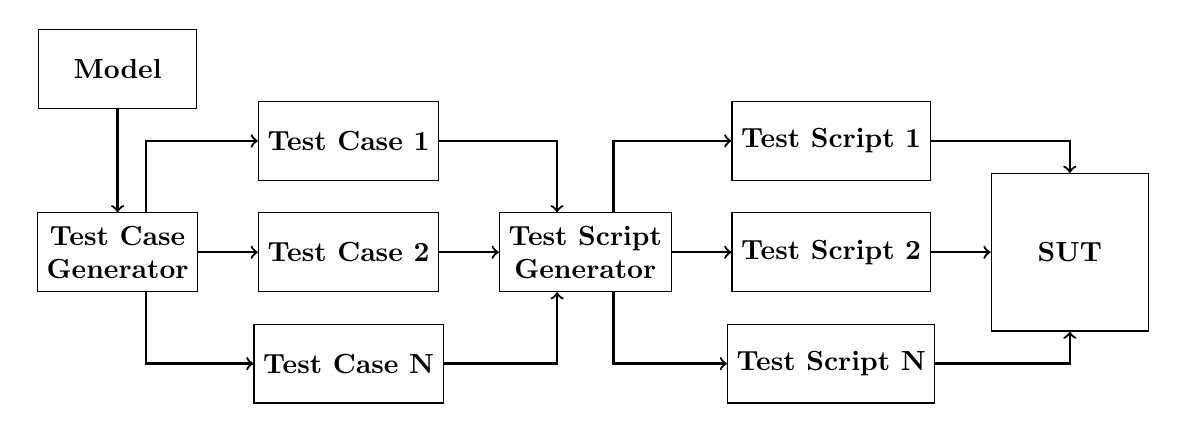
\begin{tikzpicture}
\matrix [column sep=7mm, row sep=-1mm] {
  & & & \\
  \node (model) [draw, shape=rectangle,
  minimum width=2cm, minimum height=1cm] {\textbf{Model}}; \\ 
  &  \node (tcase1) [draw, shape=rectangle,minimum width=2cm,
  minimum height=1cm] {\textbf{Test Case 1}}; & &
  \node (tscript1) [draw, shape=rectangle,minimum width=2cm,
  minimum height=1cm] {\textbf{Test Script 1}}; \\
  \node (tcasegen) [draw, shape=rectangle,
  minimum width=2cm, minimum height=1cm, align=center] {\textbf{Test Case} \\ \textbf{Generator}}; & \node (tcase2) [draw, shape=rectangle,
  minimum width=2cm, minimum height=1cm] {\textbf{Test Case 2}}; & \node (tscriptgen) [draw, shape=rectangle,
  minimum width=2cm, minimum height=1cm, align=center] {\textbf{Test Script} \\ \textbf{Generator}}; &
  \node (tscript2) [draw, shape=rectangle,minimum width=2cm,
  minimum height=1cm] {\textbf{Test Script 2}}; &
  \node (sut) [draw, shape=rectangle, minimum width=2cm,
  minimum height=2cm] {\textbf{SUT}}; \\
  & \node (tcasen) [draw, shape=rectangle,minimum width=2cm,
  minimum height=1cm] {\textbf{Test Case N}}; & &
  \node (tscriptn) [draw, shape=rectangle,minimum width=2cm,
  minimum height=1cm] {\textbf{Test Script N}}; \\
  & & \\
};
\draw[->, thick] (model) -- (tcasegen);
\draw[->, thick] (tcasegen) -- (tcase2);
\draw[->, thick] ([xshift=10mm]tcasegen) |- (tcase1);
\draw[->, thick] ([xshift=10mm]tcasegen) |- (tcasen);
\draw[->, thick] (tscriptgen) -- (tscript2);
\draw[->, thick] ([xshift=10mm]tscriptgen) |- (tscript1);
\draw[->, thick] ([xshift=10mm]tscriptgen) |- (tscriptn);
\draw[->, thick] (tcase1) -| ([xshift=-10mm]tscriptgen);
\draw[->, thick] (tcase2) -- (tscriptgen);
\draw[->, thick] (tcasen) -| ([xshift=-10mm]tscriptgen);
\draw[->, thick] (tscript1) -| (sut);
\draw[->, thick] (tscript2) -- (sut);
\draw[->, thick] (tscriptn) -| (sut);



\end{tikzpicture}
\caption{A fully automated model-based testing approach.} \label{fig:f1}
\end{figure}

After the test generation from the model and the execution of those tests against the system, each test that fails will point either to an error in the implementation of the system or to a mistake in the model. The value of model-based testing comes from the automated cross-checking between the model and the system implementation.

\subsection{Challenges in Modeling}
Model-based testing can improve considerably the test 
efficiency and test quality when the models are light 
and available. The elaboration of a model is, probably, 
the key for the success of model-based testing in practice,
and if done wrongly~\cite{Peleska.2013} can lead to a set of undesirable 
outcomes:

\begin{itemize}
\item If complex models have to be completed before testing
can start, this induces an unacceptable delay for the
proper test executions;
\item For complex SUT, like systems of systems, test models 
need to abstract from a large amount of detail, because 
otherwise the resulting test model would become unmanageable;
\item The required skills for test engineers writing test 
models are significantly higher than for test engineers 
writing sequential test procedures.
\end{itemize}

\subsection{How to execute the test suite?}

There are four types of test execution in model-based testing. The test
execution can be:
\begin{itemize}
\item \textbf{Manual}: a tester must execute each generated test case by
interacting with the system under test, following the instructions provided by
the generated test case and documenting the results. It is possible to execute
the tests without using a tool.
\item \textbf{Automated}: requires tool support and implies that the
generated test is already an executable test script. It has well-known
advantages over manual execution. The tests are faster to run, are less
expensive to repeat, and work over night without asking for a bonus. Once
written, they are continuously executed.
\item \textbf{Online}: where tests are executed as they are generated, so the
model-based testing tool is tightly coupled to the system under test. It is
particularly good for testing nondeterministic systems and for long-running test
sessions, such as overnight testing based on random traversal of a model. This
kind of technique is sometimes necessary if the system under test is
non-deterministic, because the test generator can see which path the system has
taken, and follow the same path in the model. Online model-based testing is
fully automated.
\item \textbf{Offline}: decouples the generation and execution phases, so the
test execution can be completely independent of the model-based test generation
process since the test cases are generated strictly before they are run. It can
perform a deeper analysis of the model to generate a small but
powerful test suite, and the generated test suite can be inspected, use
repeatedly for regression purposes, put into a test management system, and so on.
\end{itemize}.

Online model-based testing has the advantage of being able to deal with
nondeterministic dynamic behavior of the system under test. It is able to
produce instant results for both test generation and execution~\cite{Kramer2016}.
It is even possible to exercise very long tests, which allows you to dive deeply
into the expected behavior of the system under test.

On the other hand, the advantages of offline testing, are mostly pragmatic. The
generated tests can be managed and executed using existing test management tools,
which means that less changes to the test process are required. One can generate
a set of tests once, then execute it many times on the system under test. Also,
the test generation and test execution can be performed on different
machines or in different environments, as well as at different times. Finally,
if the test generation process is slower than test execution, then there are
obvious advantages to doing the test generation phase just once.

\subsection{Prerequisites of Model-Based Testing}

It is important to have some high-level management support for the adoption of model-based testing, as well as some enthusiasm for model-based testing among the team who will put it into practice.

Model-based testing tools implies that the test execution phase is already automated. So, for a testing team who has little experience with automated testing might be wise to gain experience with an automated approach like data or keyword-driven testing before using model-based testing.

Model-based testing models are more precise than most UML models and require detailed modeling of the system behavior. Developing these kinds of models is more similar to programming than to designing use cases and class diagrams. It is helpful to have some experience with designing interfaces and choosing good levels of abstraction.

Sometimes, model-based testing does not suit the system needs. If the system has to be tested manually because the test steps require human interaction, then the cost of that manual testing may dominate any cost savings of model-based testing.

\subsection{Model-Based Testing and Agile methods}

In terms of industrial adoption, model-based testing needs to be adapted to the
existing testing processes that are shifting towards more agile practices
from the traditional ones based on the V-model and its variations. In agile
contexts, on the one hand, developers are already relying on test automation to
support refactoring and generally understand its benefits as compared to manual
testing.

In the eyes of the agile practitioners, writing acceptance tests
that specify what the system is supposed to do, brings lot of value:
\begin{itemize}
\item It forces the customer to specify precisely what is required;
\item When the acceptance tests pass, the customer has much more confidence on
the work that has been done;
\item An executable specification gives a clear and measurable 
objective to the development team.
\end{itemize}

\noindent Having the acceptance tests centered around a model makes not only
easier to develop a significant number of acceptance tests, but also to change
the model and regenerate those same tests. We can benefit even more from mixing
model-based and acceptance tests if the model itself is built around some agile
principles. The test models should:
\begin{itemize}
\item be light; 
\item have a precise purpose;
\item grow incrementally through an iterative approach;
\item encourage discussion about the exact behavior of the system;
\end{itemize}

\subsection{Advantages of Model-Based Testing}
Model-based testing can have a small cost-benefit over keyword-based testing and a significant cost-benefit over the other testing processes~\cite{1200168}.

It can lead to less time and effort spent on testing if the time needed to write and maintain the model plus the time spent on directing the test generation is less than the cost of manually designing and maintaining a test suite. 

The use of an automated test case generator based on algorithms and heuristics to choose the test cases from the model makes the design process systematic and repeatable and it is very easy to generate more tests.

Quantity means nothing if we loose the quality of the test
suite. Several studies have shown that the use of a
model-based approach tends to increase fault detection effectiveness~\cite{Dalal1999,Farchi2002}. It is usual to find numerous faults in the requirements and design documents as a side-effect of modeling~\cite{1200168}. The detection of such faults at an early stage is the major benefit of model-based testing.

\subsection{Disadvantages of Model-Based Testing}

In spite of all of the advantages stated above, the industrial adoption of this technology has been slow. The most common problems are the managerial difficulties, the making of easy-to-use tools, the reorganization of the work with the tools~\cite{Robinson2013} and the complexity of the solutions and counter-intuitive modeling~\cite{Jääskeläinen2008}. Model-based testing is a disruptive approach to testing and needs to be managed as such. It requires changes to the way teams work and enables a total testing transformation~\cite{Jorgensen2017}.

One of the fundamental limitations~\cite{1200168} of model-based testing is that it cannot guarantee to find all the differences between the model and the implementation, not even if there are hundreds of test cases being generated by the system model.

Model-based testing is not as trivial as other testing techniques, and requires a steep learning curve and different testing skills: modeling and programming skills. It is desirable to have a reasonably mature testing process and some experience with automated test execution before fully adopt this approach.

Up to date requirements plays a big role in model-based testing. The test cases are very coupled to the requirements, and requirements change, often. If the model is build based on outdated requirements, it will lead to unreliable results and one of these tests fails, it's hard to check if the failure is caused by the system under test, the driver, or even from the model itself. This process makes more difficult and time-consuming to find the root cause of the failing test.

\newpage
Since this approach can generate huge numbers of tests, it becomes necessary to move toward other measurements of test progress instead of relying on the number-of-tests metric.

\begin{figure}[!htb]
\centering
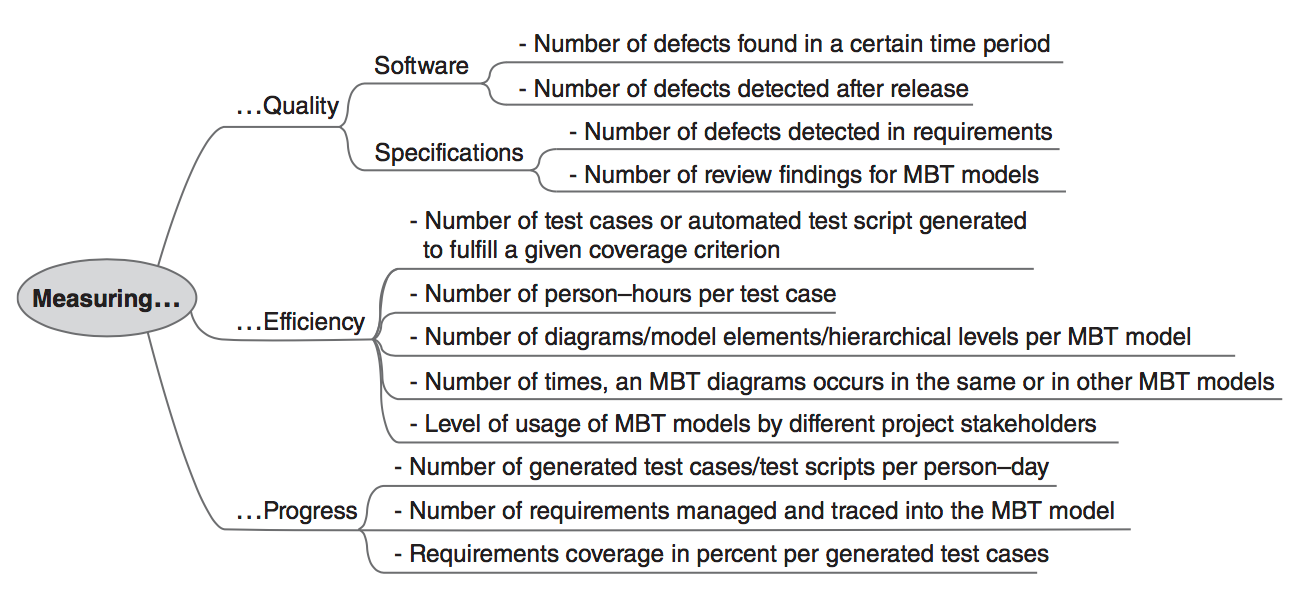
\includegraphics[scale=0.5]{metrics.png}
\caption{Possible measures for model-based testing metrics~\cite{Kramer2016}.} \label{fig:metrics}
\end{figure}

\section{Comparison between discussed techniques}

\begin{table}[!ht]
\centering
\begin{tabular}{l|p{55mm}|p{55mm}}
\textbf{Approach} & \textbf{Advantages} & \textbf{Disadvantages} \\
Data-driven
  & Easy to implement and maintain.
  & Needs skilled resources to implement the test scripts. \\
Keyword-driven
  & Tool independent and highly scalable.
  & Needs skilled resources to implement the test scripts.
    Driver an test scripts could become too complex. \\
\hline
Hybrid-driven
  & Combines the advantages \newline from all of the approaches above
  & It tend to be more complex since \newline it combines all of the approaches above.\\
\hline
Model-based
  & Model reuse, automatic test generation and higher fault detection.
  & It's too complex when comparing with the approaches above.
    Needs skilled resources to model the system. \\
\end{tabular}
\caption{Comparison between data-driven, keyword-driven, hybrid-driven, and
  model-based testing.}
\label{table:comparison-between-approaches}
\end{table}

The improved maintainability of test scripts is a strong argument in favor of
data-driven and keyword-driven test automation approaches~\cite{Kramer2016}.

In data-driven scripting, the scripts are parameterized and the concrete test
data values are recorded in a data table, that could be a database or even a
spreadsheet file. These parameterized scripts are easier to maintain, but
changing the implementation may affect a larger number test scripts.

In keyword-driven testing, scripts are structured programming constructs
based on keywords and the use of keywords separates the test logic from test
data and implementation. This way, the interface implementation can change,
leaving the test scripts with the keywords unchanged. The only thing that needs
to be modified is the concrete implementation of the adapter. This approach
minimizes source code redundancy and maintenance effort.

Model-based testing supports data-driven and keyword-driven test automation
approaches and takes the concept of abstraction even further. In the model-based
approach, there are no maintenance of individual test scripts. Instead, the
changes are directly performed in both model and adapter layer. It moves the
maintenance of the test scripts to a higher abstraction level, since the model
provides a graphical and abstract representation of them. Using a test generator
tool, the test scripts are updated in an automated process and tests cases can
be regenerated whenever required.

In practice, the model-based testing model contains action words instead of
detailed test actions from the keyword-driven approach, and equivalence
partitions and logical operators instead of concrete values for input data and
expected results from the data-driven approach.

Choosing the right framework, always depends on the project, the maturity of the
team, and the available resources.
